
%%%%%%%%%%%%%%%%%%%%%%%%%%%%%%%%%%%%%%%%%%%%%%%%%%%%%%%%%%%%%%%%%%%%%%%%%%%%%%%
%%%%%%%%%%%%%%%%%%%%%%%%%%%%%%%%%%%%%%%%%%%%%%%%%%%%%%%%%%%%%%%%%%%%%%%%%%%%%%%
%%%%%%%%%%%%%%%%%%%%%%%%%%%%%%%%%%%%%%%%%%%%%%%%%%%%%%%%%%%%%%%%%%%%%%%%%%%%%%%
\section{\textcolor{blue}{Que passos existem no samba de gafieira?}}

No ano \AnoLivro~ podemos ver uma grande variedade de passos para o samba de gafieira,
tantos como a imaginação possa atingir, pois além dos movimentos mais conhecidos e  consagrados da dança,
podem existir variações  destes ou simplesmente estilos em que estos são realizados. 



Nas seguintes subseções, listaremos e descreveremos 
alguns dos passos que são possíveis de ver no samba de gafieira;
mas, estas descrições não pretendem ser uma guia de ensino,
e sim um instrumento para saciar a curiosidade do leitor em como os movimentos são realizados.\\

%%%%%%%%%%%%%%%%%%%%%%%%%%%%%%%%%%%%%%%%%%%%%%%%%%%%%%%%%%%%%%%%%%%%%%%%%%%%%%%
%%%%%%%%%%%%%%%%%%%%%%%%%%%%%%%%%%%%%%%%%%%%%%%%%%%%%%%%%%%%%%%%%%%%%%%%%%%%%%%
\PRLsep{Passos no samba de gafieira ate 1949}
%%%%%%%%%%%%%%%%%%%%%%%%%%%%%%%%%%%%%%%%%%%%%%%%%%%%%%%%%%%%%%%%%%%%%%%%%%%%%%%
\subsection{Balão} 
\label{def:PassoBalao}
\index{Passo!Balão}
\index{Passo a contratempo!Balão}
%%                CICLICO    |SIMETRICO   |CONTRATEMPO   |DESLOCAMENTOS |TIEMPOS
\caracterpasso{\NoCheckedItem}{\NoCheckedItem}{\CheckedItem}{\NoCheckedItem}{3}
Um movimento com este nome já existia desde as origens do samba nas gafieiras, 
sendo este movimento proveniente do maxixe \cite[pp. 142]{perna2002samba} 
\cite[pp. 93]{efege1974maxixe} \cite[pp. 465]{marcondes1977enciclopedia}.
%porem não tem se achado referencias sobre as caraterísticas do movimento no maxixe.



Seguindo o Prof. Gino Fornaciari, no ano 1947,  em São Paulo, se usava o nome balão e pião,
para representar a um mesmo movimento, um que agora chamaríamos de pião, 
porem o pião de 1947 era em sentido anti-horário \cite[pp. 68-72]{fornaciari1947aprender}.
Por outro lado, no seu livro ``Como apender a dançar'' (1950) 4ta edição,
o Prof. Fornaciari descreve um movimento  chamado ``Calçada'', com uma descrição semelhante 
ao ``balão'' de \AnoLivro~ \cite[pp. 162]{fornaciari1950aprender}.

Em \AnoLivro, o nome balão designa a um movimento que pode ser considerado aéreo, 
pois o \hyperref[def:Condutor]{\textbf{condutor}} tira do chão os pés do \hyperref[def:Seguidor]{\textbf{seguidor}}.
Um movimento com estas caraterísticas pode ser visto no filme ``Aviso aos navegantes'' (1950),
pelo que podemos especular que este era de uso comum desde muito antes \cite[min. 40:35]{AtlantidaDance};
porem, não pode-se souber sim lhe era atribuído ou não nessa época o nome de balão; 
mas pela semelhança com o movimento de quadril do passo chamado balão apagado,
é provável que sim, 
pois lembremos que o problema da homologação da nomenclatura dos passos existe ate em  nossos dias.



O movimento dura 3 tempos, o passo inicia com o seguidor ao lado direito do condutor, 
ligeiramente atrás dele, com um \hyperref[def:abracodedanca]{\textbf{abraço de dança}} 
bem próximo e uma postura similar à \hyperref[def:X-position]{\textbf{posição de X}} só que com os pés mais juntos.
No primeiro tempo o condutor da um passo ao lado, e pisa com o pé direito,
de modo que o seguidor fique em pé atrás da perna direita do condutor, sem perder o abraço.
No segundo tempo, aproveitando a postura, 
o condutor faz um movimento circular anti-horário com seu quadril, no \hyperref[def:PlanoAxial]{\textbf{plano axial}},
de modo que sua perna direita, que está em contato com a perna direita do seguidor,
serva como alavanca para tirar ao seguidor do chão, 
e este gire ou voe ao redor \footnote{O giro do seguidor é com o corpo reto e pernas juntas, 
como se fosse uma fita solta de um lado e com o outro lado presso num ponto 
que provoca o giro da fita no \hyperref[def:PlanoAxial]{\textbf{plano axial}}, com giro ao redor do eixo axial.} 
do condutor em sentido anti-horário.
No terceiro tempo o seguidor senta-se, é dizer faz uma cadeirinha, sobre a perna esquerda do condutor,
que para receber ao seguidor  da um passo ao frente.

\begin{comment}
A Figura \ref{fig:balao1950} mostra um fotograma do filme ``Aviso aos navegantes'' (1950),
onde se observa o inicio do passo balão (\AnoLivro), quando a moça tira os pés do chão.
\begin{figure}[h!]
  \centering
    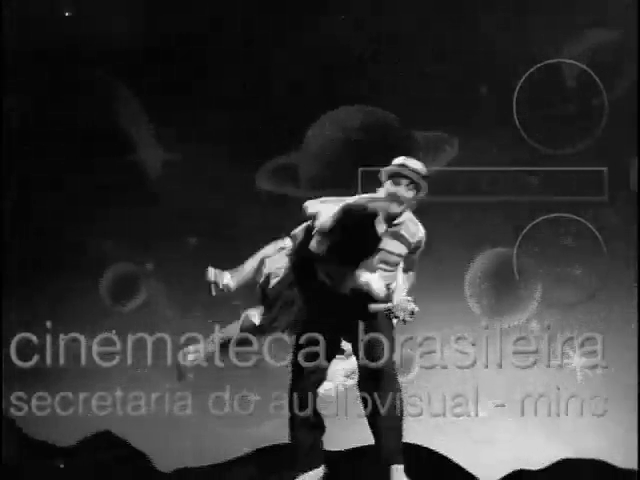
\includegraphics[width=0.7\textwidth]{chapters/cap-historia-passos/balao1950.png}
  \caption{Fotograma com o inicio do passo balão (\AnoLivro), do filme ``Aviso aos navegantes'' (1950) \cite[min. 40:35]{AtlantidaDance}.}
  \label{fig:balao1950}
\end{figure} 
\end{comment}

%%%%%%%%%%%%%%%%%%%%%%%%%%%%%%%%%%%%%%%%%%%%%%%%%%%%%%%%%%%%%%%%%%%%%%%%%%%%%%%
\subsection{Balão apagado}
\index{Passo!Balão apagado} 
\index{Passo cíclico!Balão apagado}
\index{Passo simétrico!Balão apagado}
%%                CICLICO     |SIMETRICO   |CONTRATEMPO   |DESLOCAMENTOS |TIEMPOS
\caracterpasso{\CheckedItem}{\CheckedItem}{\NoCheckedItem}{\NoCheckedItem}{4}
Um movimento com este nome já existia desde as origens do samba nas gafieiras, 
sendo este movimento proveniente do maxixe \cite[pp. 142]{perna2002samba} \cite[pp. 68]{efege1974maxixe}.
Um exemplo do movimento que agora designamos como balão apagado pode 
ser visto no filme ``Aviso aos navegantes'' (1950) \cite[min. 40:35]{AtlantidaDance}.
\begin{comment}
A Figura \ref{fig:balaoapagado1950} mostra um fotograma do filme onde se observa o movimento de quadril no balão apagado.
\begin{figure}[h!]
  \centering
    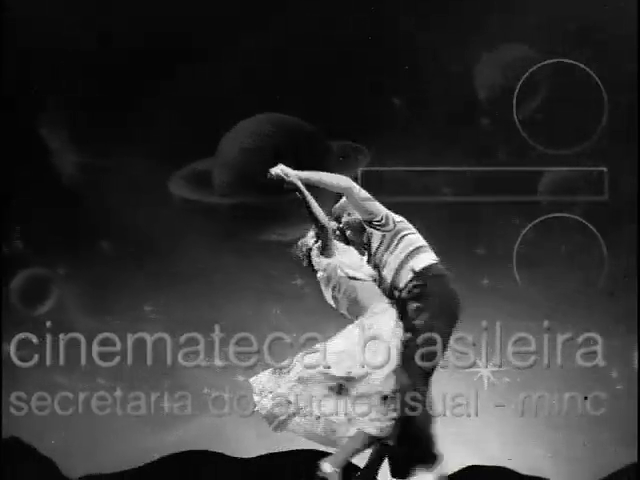
\includegraphics[width=0.7\textwidth]{chapters/cap-historia-passos/balaoapagado1950.png}
  \caption{Fotograma que mostra a execução do passo balão apagado, tirado do filme ``Aviso aos navegantes'' (1950) \cite[min. 40:35]{AtlantidaDance}.}
  \label{fig:balaoapagado1950}
\end{figure}
\end{comment}

Em \AnoLivro, este movimento tem um parecido ou lembrança com o \hyperref[def:PassoBalao]{\textbf{balão}} (\AnoLivro); 
porem, se realiza com o par num \hyperref[def:abracodedanca]{\textbf{abraço de dança}} estando um frente ao outro, 
consequentemente o \hyperref[def:Seguidor]{\textbf{seguidor}} não voa ao redor do \hyperref[def:Condutor]{\textbf{condutor}}, 
se não que a intenção de voar se apaga e o seguidor nunca sai do chão; 
de modo que o casal fica dando giros, abraçados, num eixo comum e praticamente no lugar. 
Estes giros são promovidos por marcados movimentos circulares de quadril, que mudam
de velocidade e intenção num constante, abrupto, leve e leve,  na proporção de tempos \{1/2 tempo,1/2 tempo, tempo\}; 
semelhando assim ao movimento de um balão perdendo o ar.
Existem variantes deste movimento, onde o giro do par é realizado em sentido horário e anti-horário; porem, 
não saberia afirmar qual é a versão padrão; mas, pelas minhas observações a versão mais difundida,
é a que faz o giro em sentido anti-horário.

Este movimento é um \hyperref[def:PassoCiclico]{\textbf{passo cíclico}}, com ciclos que duram 4 tempos, 
sendo o primeiro par de tempos similar ao segundo, porem com os papeis intercambiados no par de dança.
No momento inicial, o casal está abraçado numa \hyperref[def:frente-frente-position]{\textbf{posição frente a frente}}, 
com o peso do corpo do lado da perna direita do condutor;
no tempo 1 o condutor da um passo e pisa com a perna esquerda pra traz, 
como se procura-se ocultar esta atrás da sua perna direita, 
este movimento de perna é promovido pelo movimento circular do 
quadril em sentido anti-horário no \hyperref[def:PlanoAxial]{\textbf{plano axial}};
por outro lado, 
o seguidor da um passo adiante com sua perna direita procurando manter a postura 
relativa com o condutor e acompanhando o movimento circular anti-horário do quadril, 
de modo que se seu pé direito tende a   rodear ao condutor.
Nos tempos 1.5 e 2 o par pisa no lugar, ajeitando suas posturas apagando o movimento do quadril, 
mas mantendo o giro do par, 
de modo que terminam abraçados  frente a frente com o peso do corpo no lado do pé esquerdo do condutor.
No próximo par de tempos, o movimento é similar, só que agora é o seguidor que inicia dando um passo com o pé esquerdo. 

%%%%%%%%%%%%%%%%%%%%%%%%%%%%%%%%%%%%%%%%%%%%%%%%%%%%%%%%%%%%%%%%%%%%%%%%%%%%%%%
\subsection{Puladinho }
\index{Passo!Puladinho}
\index{Passo cíclico!Puladinho}
\index{Passo simétrico!Puladinho}
\index{Passo de deslocamento!Puladinho}
\begin{comment} 
neste movimento não se pula; 
existem varias referencias não acadêmicas na internet, que datam desde o 2002,
onde não mencionam ao ``Puladinho'' e sim um passo chamado ``pruladinho'', 
pelo qual suspeito que este faz referencia ao mesmo passo;
pois indica corretamente que no movimento se vá ``pra o ladinho''.
\end{comment}

Na polca, trazida ao Brasil em 1845, 
existia um movimento chamado puladinho,
que era um movimento que se fazia sobre as pontas dos pés,
indo para adiante, iniciando com o pé esquerdo estacando obliquamente à esquerda,
num segundo momento o pé direito avança ate ficar junto ao outro, 
para logo deslizar o pé esquerdo para adiante, 
permitindo assim levantar o pé direito para ajeitar a postura 
e recomeçar o movimento com esquerdo \cite[pp. 58-59]{tinhorao1986pequena}.
É fácil perceber que este movimento tem alguns pontos semelhantes ao puladinho (\AnoLivro),
no fato do andar oblíquo e a troca de pesos, porem o puladinho da polca não era simétrico para ambos pés.

%%                CICLICO     |SIMETRICO   |CONTRATEMPO   |DESLOCAMENTOS |TIEMPOS
\caracterpasso{\CheckedItem}{\CheckedItem}{\NoCheckedItem}{\CheckedItem}{4}
Por outro lado, no maxixe (dança)  que é descrito em 1920 na ``Revista do Brasil'',
se mencionam os termos maxixe ``puladinho'' e maxixe de ``esquentar a barriga'',
como descrições usadas pelos aficionados a esta dança, 
pelo que se entende que no maxixe também existiu um movimento chamado puladinho \cite[pp. 177]{1920revista}. 

Adicionalmente, no livro ``Oito décadas: memórias'', se menciona que na década de
1920 existia uma variante do samba que se chamava ``o puladinho'' 
que introduziu nos salões o carnaval do povo, 
e que provocava entre as jovens da época, em palavras da autora, 
``a externalização da sensualidade reprimida'' \cite[pp. 94-95]{nabuco2000oito}.

Conhecidas estas informações, é importante lembrar que a polca influenciou a criação do maxixe (dança), 
que a sua vez influenciou a criação do samba dançado nas gafieiras,
que se condensou no samba de gafieira (\AnoLivro), o qual tem em nossos dias um passo chamado puladinho. 
Pelo que pode-se considerar, pela existência do termo em todas as evoluções da dança; 
que um movimento chamado puladinho 
já estava também presente nos primeiros sambas dançados nas gafieiras. 

Reforçando esta hipótese, podemos achar uma referencia ao uso do termo puladinho, no título de uma música instrumental chamada 
``Puladinho na gafieira'' (1958)  de  Marisa com Moacyr Silva e seu conjunto: Convite à música \cite{puladinhogafieiramusic}.
Também, podemos ver uma menção a este movimento, junto a outros conhecidos no samba de gafieira,
em 1976 na revista ``Veja'' \cite[pp. 158]{1976veja},
em 1978 na letra da canção ``Baile no Elite'' \cite{BaileNoElite} e 
em 1979 na revista ``Isto é'' \cite[pp. 89]{revista1979isto}.



Finalmente, podemos ver uma referencia a esse passo de dança, no ``jornal dos sports''(RJ),
do dia 17 de julho de 1986 \cite[pp. 6]{gafieiraaredeout2}.


O puladinho, de \AnoLivro, é executado com o casal abraçado frente a frente, sendo este um \hyperref[def:PassoCiclico]{\textbf{passo cíclico}},
com uma duração de 4 tempos; onde o movimento dos dois primeiros tempos
é simétrico ao segundo par de tempos.
Desde o ponto de vista do  \hyperref[def:Condutor]{\textbf{condutor}}, 
este inicia o movimento levando o peso do corpo junto com seu pé direito para atrás, provocando que
o \hyperref[def:Seguidor]{\textbf{seguidor}} de um passo ao frente acompanhando-lhe;
porem o condutor realiza seu movimento predominantemente pela ação do quadril e com um ligeiro arco para a direita, 
com o fim de dar molejo ao movimento;
no tempo 1.5 sem deslocar os pés, 
se faz uma troca de peso do corpo para o pé esquerdo do condutor (direito do seguidor) usando o quadril,
e finalmente no tempo 2 o condutor volta a levar o peso 
do corpo para a sua perna direita (esquerdo do seguidor) novamente usando o quadril.
Neste ponto a metade do ciclo foi realizado e o movimento se repete simetricamente, 
de modo que no tempo 3 o condutor leva atrás o seu pé esquerdo (direito do seguidor) e continua em 3.5 e 4.

 
%%%%%%%%%%%%%%%%%%%%%%%%%%%%%%%%%%%%%%%%%%%%%%%%%%%%%%%%%%%%%%%%%%%%%%%%%%%%%%%
\subsection{Pião}
\index{Passo!Pião}
\index{Passo cíclico!Pião}
\index{Passo simétrico!Pião}
\index{Passo de deslocamento!Pião}

Seguindo o Prof. Gino Fornaciari, no ano 1947,  em São Paulo, os nomes pião e balão,
representavam ao mesmo movimento, no samba-batucada\footnote{Samba de gafieira primigeinio.}; 
porem o pião de 1947 era em sentido anti-horario \cite[pp. 68-72]{fornaciari1947aprender}.
Também, podemos ver uma menção a este movimento, junto a outros conhecidos no samba de gafieira, 
em 1979 na revista ``Isto é'' \cite[pp. 89]{revista1979isto}.
Todas estas afirmações são coerentes com as declarações de Jimmy de Oliveira 
que indica que o pião já existiam antes do 1990 \cite{sambafunkeadoJimmyDeOliveiraPart1}.

%%                CICLICO     |SIMETRICO   |CONTRATEMPO   |DESLOCAMENTOS |TIEMPOS
\caracterpasso{\CheckedItem}{\CheckedItem}{\NoCheckedItem}{\CheckedItem}{4}
O pião, de \AnoLivro, é um \hyperref[def:PassoCiclico]{\textbf{passo cíclico}} que é executado com o casal abraçado, 
realizando giros sobre um eixo comum.
Cada giro dura 2 tempos, e é realizado tradicionalmente em sentido horário;
na primeira metade do giro (que dura 1 tempo) o eixo de giro do par é colocado sobre uma pessoa do par, 
de modo que a outra pessoa gira ao redor (em 1 tempo), ate chegar a uma postura similar à inicial, 
porem com os papeis intercambiadas no par, com respeito ao tempo anterior;
na outra metade do ciclo se repete o movimento, porem agora é a outra pessoa que terá o eixo do par.
Este é um movimento de deslocamento, de modo que se procura girar movimentando-se numa linha reta.

%%%%%%%%%%%%%%%%%%%%%%%%%%%%%%%%%%%%%%%%%%%%%%%%%%%%%%%%%%%%%%%%%%%%%%%%%%%%%%%
\subsection{Pica-pau} 
\index{Passo!Pica-pau}
\index{Passo cíclico!Pica-pau}
\index{Passo simétrico!Pica-pau}

%%                CICLICO     |SIMETRICO   |CONTRATEMPO   |DESLOCAMENTOS |TIEMPOS
\caracterpasso{\CheckedItem}{\CheckedItem}{\NoCheckedItem}{\NoCheckedItem}{4}
Nos primórdios do samba nas gafieiras existia um passo de dança com esse nome \cite[pp. 142]{perna2002samba}.
No Fandango\footnote{Para mais informação sobre o fandango, ir a Pag. \pageref{fig:fandango}.} 
rufado-bailado de São Paulo, em 1948, existiu uma dança chamada ``pica-pau'';
%com uma coreografia semelhante ao ``anucorrido'' (anu-corrido);
em Itanhaém (SP) esta dança é caraterizada por pares espalhados no salão,
onde o canto do violeiro é alternado com batidas de pé e palmas pelos 
cavalheiros \cite[pp. 607-608]{marcondes1977enciclopediav2} \cite[pp. 49]{fandangoSP},
esta caraterística do uso dos pés é o que da uma semelhança ao pica-pau do samba de gafieira (\AnoLivro),
que leva esse nome porque se bate o chão com a ponta (ou meia ponta) do pé simulando as bicadas de um pássaro pica-pau.
Porem, a existência do pica-pau no fandango não indica uma relação de vinculo parental do movimento,
e sim que no consciente coletivo, o estilo de imitar ao pica-pau, na dança,
já estava presente desde antes dessa época.
Um movimento com as caraterísticas do pica-pau (\AnoLivro) pode ser visto 
no filme ``Aviso aos navegantes'' (1950) \cite[min. 40:35]{AtlantidaDance}.


No \AnoLivro, o passo pica-pau, é um \hyperref[def:PassoCiclico]{\textbf{passo cíclico}} que dura 4 tempos, 
sendo os dois primeiros simétricos aos dois últimos, 
onde no primeiro par de tempos se usa só um pé,
e no segundo o outro.
Se iniciamos com o peso do corpo na perna esquerda, 
no tempo 1 marcamos com o pé direito, um pouco atrás do pé esquerdo, 
com a ponta ou meia ponta do pé e sem levar o peso,
no tempo 1.5 repetimos o mesmo movimento com o mesmo pé, e finalmente
no tempo 2 colocamos o pé direito ao lado e a direita do pé esquerdo, 
levando esta vez o peso do corpo. 
Nos tempo 3, 3.5 e 4 se repete o movimento explicado anteriormente; porem,
agora se usa o pé esquerdo.
  
\begin{figure}[t]
\begin{elaboracion}[title=Fandango]
Esta é a designação que se lhe dá a todas as danças de 
roda para adultos, em São Paulo, Paraná, Santa Catarina e Rio Grande do Sul;
este termo para eles significa baile rural ou popular \cite[pp. 261]{marcondes1977enciclopedia}.
No litoral paulista, em 1948, o Fandango é dividido principalmente em duas categorias: Fandango rufado, 
e Fandango bailado (ou valsado), porem existe a possibilidade de 
misturar e fazer um Fandango rufado-bailado \cite[pp. 48-49]{fandangoSP}.
O Fandango rufado é um conjunto de danças em que se usam batidas de pé e palmas, 
que exigem do dançarino muita energia; exemplos: O ``Chico'', ``Sapo'', 
``Farrabio'' ou ``Sarrabalho'', ``Vilão'', ``Querumana'', ``Anu-velho'', ``Recortado'' \cite[pp. 48-49]{fandangoSP}, 
etc.
O Fandango bailado é um conjunto de danças onde  não entram batidas de pé e palmas,
este é dançado dentro de casa quando os dançarinos estão cansados ou com menos energia;
exemplos: O ``Manjericão'', ``Faxineira'', ``Chamarrita'', ``Graciana'', ``Dandão'' \cite[pp. 49]{fandangoSP}, 
etc.
No Fandango rufado-bailado existem partes onde se dão batidas de pés e outras de deslisamentos e giros de valsa;
exemplos: O ``Pipoca'', ``Anucorrido'', ``Pica-pau'', ``Sinsará'' e ``Tonta'' ou ``Tontinha'' \cite[pp. 49]{fandangoSP}.
\end{elaboracion}
\label{fig:fandango}
\vspace{-20pt}
\end{figure}

%%%%%%%%%%%%%%%%%%%%%%%%%%%%%%%%%%%%%%%%%%%%%%%%%%%%%%%%%%%%%%%%%%%%%%%%%%%%%%%
%%%%%%%%%%%%%%%%%%%%%%%%%%%%%%%%%%%%%%%%%%%%%%%%%%%%%%%%%%%%%%%%%%%%%%%%%%%%%%%
\PRLsep{Passos no samba de gafieira anteriores a 1986}

\vspace{-10pt}
\subsection{Elevador}
\index{Passo!Elevador}
\label{def:PassoElevador}
\index{Passo cíclico!Elevador}
\index{Passo de deslocamento!Elevador}

%%                CICLICO     |SIMETRICO   |CONTRATEMPO   |DESLOCAMENTOS |TIEMPOS
\caracterpasso{\CheckedItem}{\NoCheckedItem}{\NoCheckedItem}{\CheckedItem}{2}
Um movimento com as caraterísticas, do que no \AnoLivro~ conhecemos como elevador, 
pode ser visto no filme ``Aviso aos navegantes'' (1950) \cite[min. 40:35]{AtlantidaDance}.
Por outro lado, na 4ta edição do livro ``Como aprender a dançar'' (1950) do Prof. Fornaciari,
podemos achar uma descrição de um movimento que no \AnoLivro~ chamaríamos de elevador \cite[pp. 161]{fornaciari1950aprender}.
Ambas referencias, descrevem de um jeito ligeiramente distinto ao movimento,
porem estas descrições nos permitem conhecer que este movimente já existia e era 
praticado antes de 1950.

No \AnoLivro, o elevador é um movimento que dura 2 tempos, e geralmente é
executado desde a \hyperref[def:facao-position]{\textbf{posição de facão}} 
estando o par num \hyperref[def:abracodedanca]{\textbf{abraço de dança}}.
Antes de iniciar o movimento o \hyperref[def:Condutor]{\textbf{condutor}} 
desce sua mão esquerda, em relação a linha dos ombros, 
para que o \hyperref[def:Seguidor]{\textbf{seguidor}}
a use de apoio para segurar o peso do corpo com sua mão direita no transcurso do movimento.
É importante ressaltar que o braço esquerdo do condutor não tenta elevar ao seguidor, 
e sim simplesmente tenta manter a postura,
o que misturado com o movimento de pernas do condutor,
provoca a saída do chão do seguidor.
No tempo 1 o condutor sai da posição de facão colocando seu pé esquerdo 
ao lado do outro, ficando em pé; dado que o condutor não deixa a postura do abraço de dança,
e este mantêm a postura da mão esquerda  como apoio ao seguidor, este é elevado, tirando os pés do chão;
no tempo 2 o seguidor desce tocando o chão, primeiro com o pé direito e logo com o esquerdo retoma a posição de facão.

É interessante ressaltar que o elevador de 1950, 
não inicia desde a \hyperref[def:facao-position]{\textbf{posição de facão}}, e 
o seguidor  não se eleva por ação do braço apoio.
Analisando o video, é ``provável'' que o seguidor seja elevado principalmente pela ação do abraço do condutor
mediante a curvatura para atrás que este faz com a parte baixa da coluna.
\begin{comment}
A Figura \ref{fig:elevador50} mostra um fotograma do filme onde se observa como o seguidor é elevado.
\begin{figure}[h!]
  \centering
    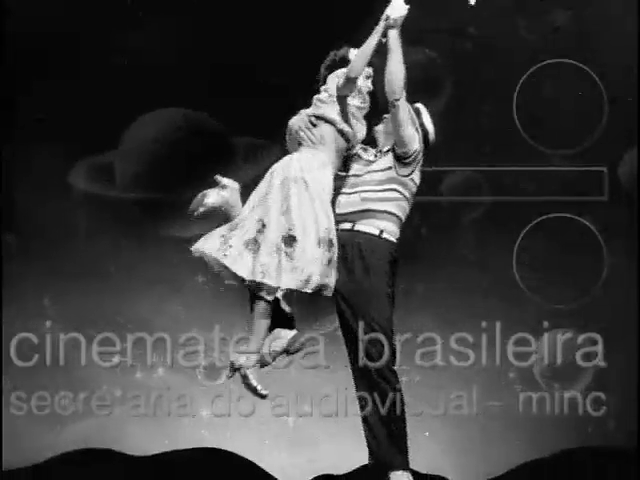
\includegraphics[width=0.7\textwidth]{chapters/cap-historia-passos/elevador1950.png}
  \caption{Fotograma do tempo 1 do passo elevador, tirado do filme ``Aviso aos navegantes'' (1950) \cite[min. 40:35]{AtlantidaDance}.}
  \label{fig:elevador50}
\end{figure}
\end{comment}



%%%%%%%%%%%%%%%%%%%%%%%%%%%%%%%%%%%%%%%%%%%%%%%%%%%%%%%%%%%%%%%%%%%%%%%%%%%%%%%
\subsection{Cruzado}
\index{Passo!Cruzado}
\index{Passo cíclico!Cruzado}
\index{Passo simétrico!Cruzado}
%%                CICLICO     |SIMETRICO   |CONTRATEMPO   |DESLOCAMENTOS |TIEMPOS
\caracterpasso{\CheckedItem}{\CheckedItem}{\NoCheckedItem}{\NoCheckedItem}{4}
Este movimento de samba de gafieira não tem uma data de criação conhecida \cite[pp. 143]{perna2002samba};
porem, podemos ver uma menção a este movimento, junto a outros conhecidos neste estilo,
em 1976 na revista ``Veja'' \cite[pp. 158]{1976veja},
em 1978 na letra da canção ``Baile no Elite'' \cite{BaileNoElite}  e 
em 1979 na revista ``Isto é'' \cite[pp. 89]{revista1979isto},
pelo que podemos estabelecer sua data de criação em algum momento anterior a 1976.
No \AnoLivro, este é um \hyperref[def:PassoCiclico]{\textbf{passo cíclico}} que dura 4 tempos;
e inicia na \hyperref[def:X-position]{\textbf{posição de X}}.
Em todo o movimento este abraço se mantêm e os dois primeiros tempos 
são simétricos aos dois últimos, porem com os pés trocados (direita por esquerda). 
Assim, no tempo 1, 
se muda a uma \hyperref[def:frente-frente-position]{\textbf{posição frente a frente}} desde a posição de X;
para conseguir isto o \hyperref[def:Condutor]{\textbf{condutor}} 
leva sua perna esquerda para a frente e o \hyperref[def:Seguidor]{\textbf{seguidor}}  a direita para atrás,
em ambos casos, os movimentos estão em referencia a seus 
respetivos \hyperref[def:PlanoFrontal]{\textbf{planos frontais}} e 
se pisa e se transfere o peso do corpo no tempo 1.
No tempo 1.5 ambos dançarinos realizam só uma transferência de peso (sem deslocamento),
o condutor para sua perna direita e o seguidor para sua esquerda.
No tempo 2 ambos dançarinos cruzam as pernas, 
o condutor cruza a perna esquerda por frente da direita, e o seguidor a perna direita por trás da esquerda.
Neste ponto o par se encontra numa postura similar a posição de X, 
com diferencia que na posição de X é a perna esquerda de ambos que fica uma próxima a outra,
e nesta última postura são as pernas esquerdas que ficam próximas.
Nos tempos 3, 3.5 e 4, se repete a essência do movimento anteriormente descrito;
é dizer, se abre a uma posição frente a frente, se ajeita o peso do corpo e finalmente se cruzam as pernas;
chegando no tempo 4 na posição de X.


%%%%%%%%%%%%%%%%%%%%%%%%%%%%%%%%%%%%%%%%%%%%%%%%%%%%%%%%%%%%%%%%%%%%%%%%%%%%%%%
\subsection{Cadeirinha}
%\index{Passo!Cadeirinha}
\index{Posição!Posição de cadeirinha}
\index{Posição de finalização!Posição de cadeirinha}

%%                FINALIZA     |TRANSIÇÂO
\caracterpostura{\CheckedItem}{\NoCheckedItem}
Uma posição com as caraterísticas do que no \AnoLivro~ conhecemos como cadeirinha, 
pode ser visto no filme ``Aviso aos navegantes'' (1950),
pelo que podemos especular que este existia desde muito antes \cite[min. 40:35]{AtlantidaDance}.
\begin{comment}
A Figura \ref{fig:cadeirinha1950} mostra um fotograma deste filme, onde se observa a cadeirinha.
\begin{figure}[h!]
  \centering
    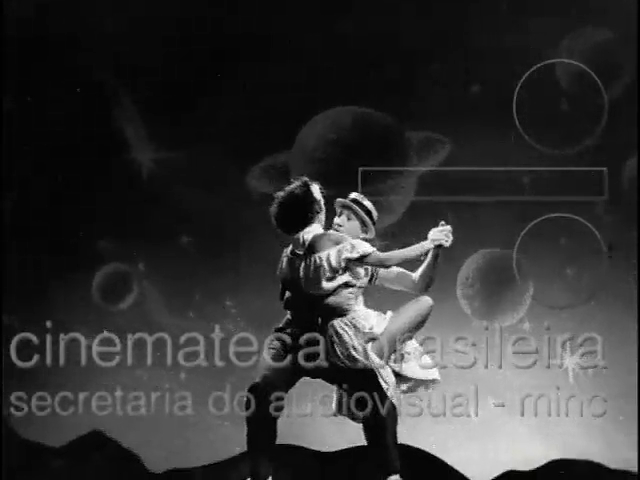
\includegraphics[width=0.7\textwidth]{chapters/cap-historia-passos/cadeirinha1950.png}
  \caption{Fotograma da cadeirinha, tirado do filme ``Aviso aos navegantes'' (1950) \cite[min. 40:35]{AtlantidaDance}.}
  \label{fig:cadeirinha1950}
\end{figure}
\end{comment}
Posteriormente, é possível achar o passo numa fotografia com a posição final caraterística da cadeirinha, 
no ``jornal dos sports''(RJ),
do dia 17 de julho de 1986 \cite[pp. 6]{gafieiraaredeout2}. 
\begin{comment}
como pode ser visto na Figura \ref{fig:cadeirinha86}.
\begin{figure}[h!]
  \centering
    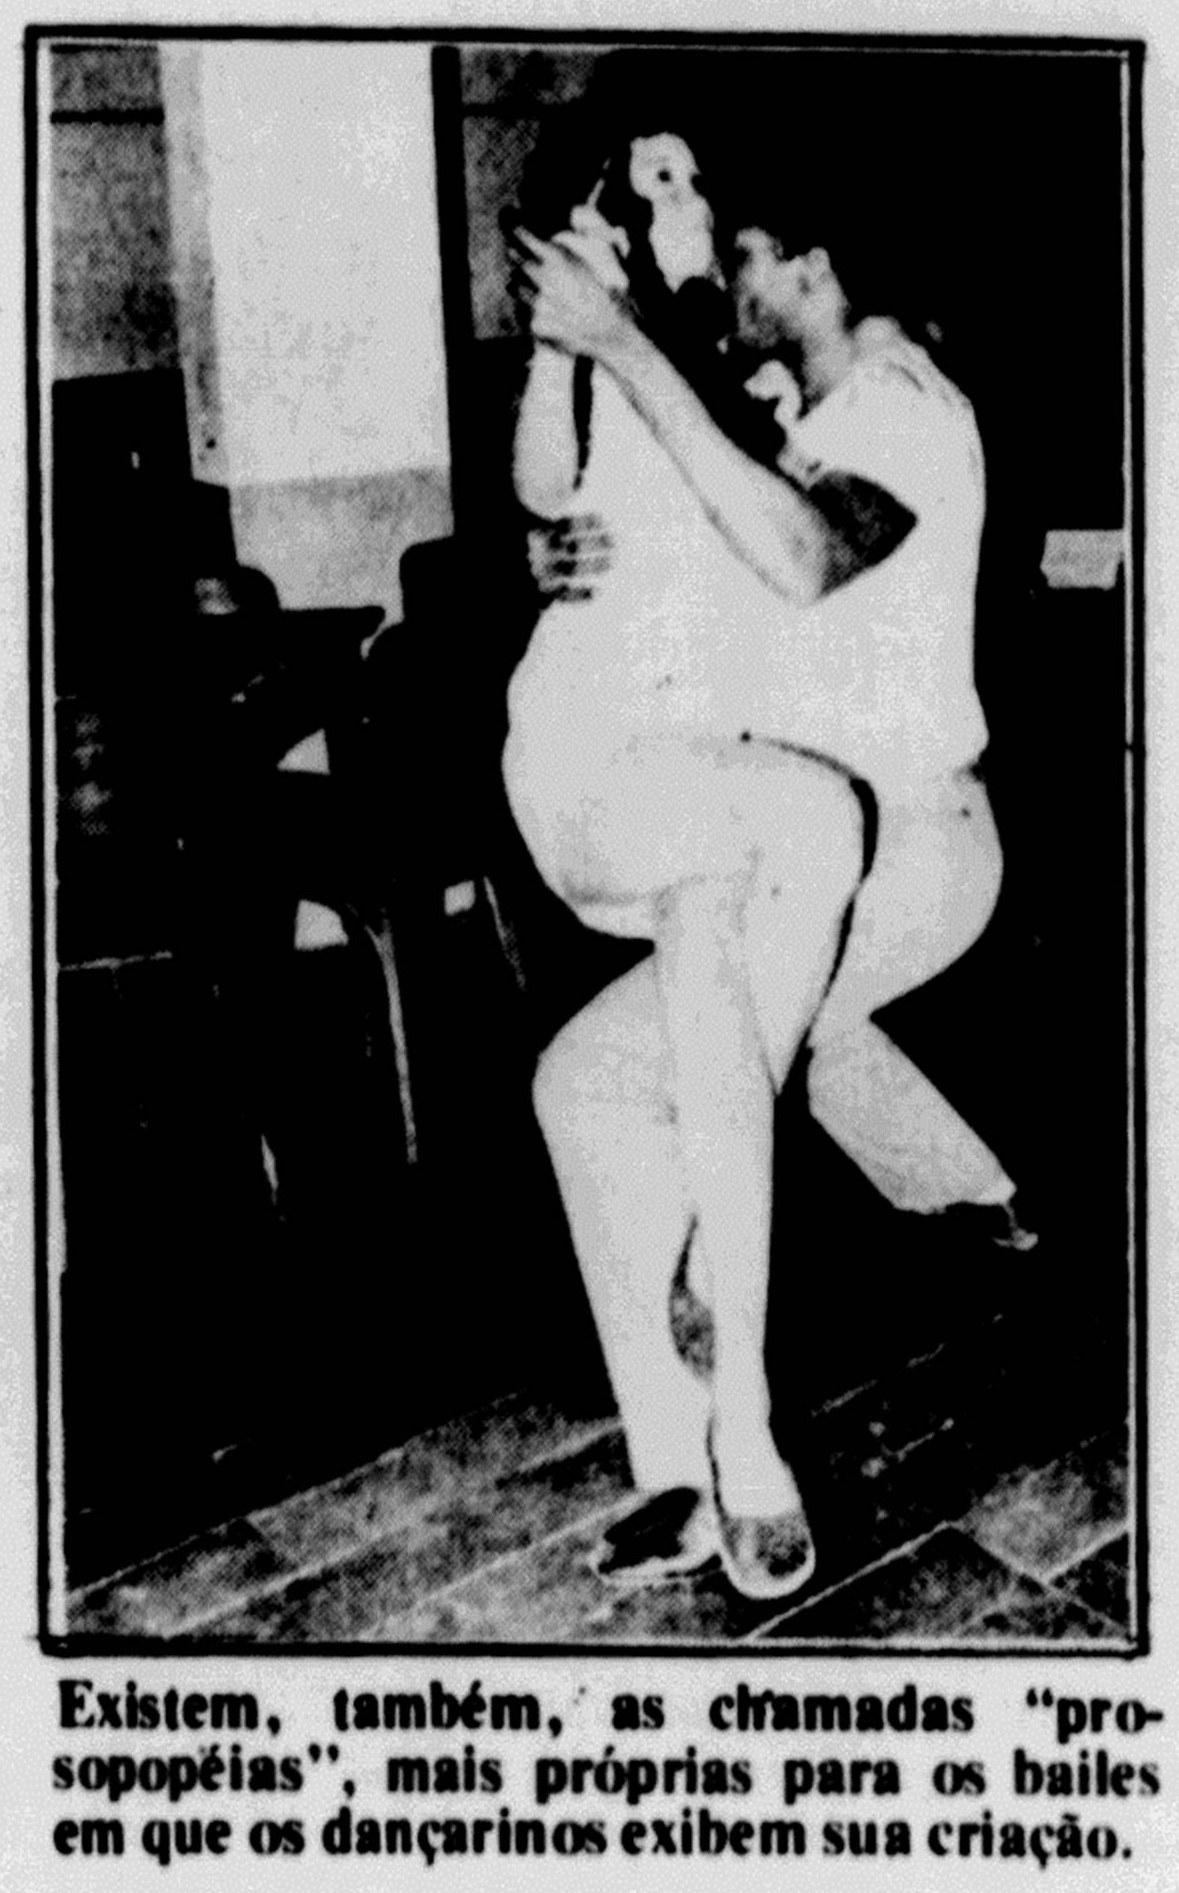
\includegraphics[width=0.45\textwidth]{chapters/cap-historia-passos/cadeirnha1986.jpg}
  \caption{Fotografia da postura da cadeirinha, publicada em 1986 no ``jornal dos sports''(RJ) \cite[pp. 6]{gafieiraaredeout2}.}
  \label{fig:cadeirinha86}
\end{figure}
\end{comment}

\begin{wrapfigure}{r}{0.25\textwidth}
  \vspace{-10pt}
  \centering
    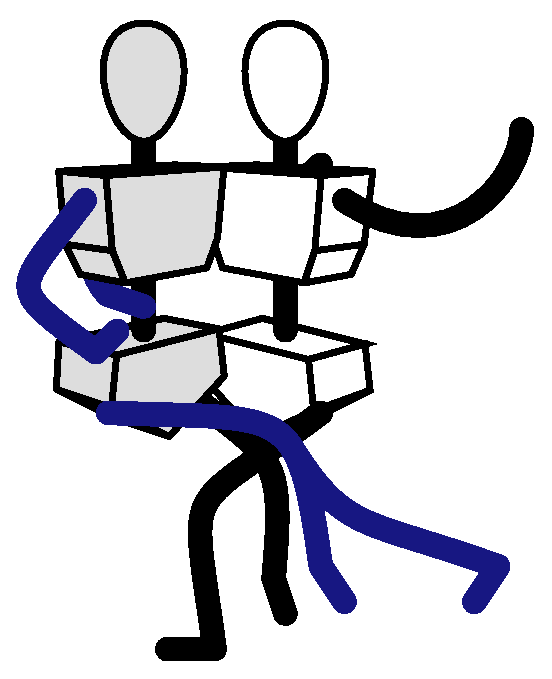
\includegraphics[width=0.23\textwidth]{chapters/cap-historia-passos/cadeirinha.eps}
  \caption{Pose final da  cadeirinha.}
  \label{fig:cadeirinhastickman}
  \vspace{-10pt}
\end{wrapfigure}
No \AnoLivro, o nome cadeirinha representa de forma particular a uma postura onde o \hyperref[def:Seguidor]{\textbf{seguidor}} 
senta-se sobre a perna do \hyperref[def:Condutor]{\textbf{condutor}}  (comumente sobre a perna esquerda);
por outro lado, de forma mais geral  o nome representa a qualquer movimento que tenha como final a 
\hyperref[def:cadeirinha-position]{\textbf{posição de cadeirinha}}.

A saída do chão do seguidor pode-se originar desde vários movimentos ou passos,
como por exemplo do  \hyperref[def:PassoBalao]{\textbf{balão}}; 
porem,
todos conservam a mesma técnica, que ao igual que  no caso do passo  \hyperref[def:PassoElevador]{\textbf{elevador}},
a suspensão no ar do seguidor, é mantida e sustentada pelo braço esquerdo do condutor,
que para este propósito  desce da linha dos ombros.
É importante lembrar que este braço não faz força para levantar ao seguidor, 
e sim simplesmente tenta manter a postura,
o que misturado com o movimento do corpo do condutor (esticar as pernas anteriormente flexionadas, principalmente)
provoca a saída do chão e suspensão do seguidor.
A Figura \ref{fig:cadeirinhastickman} mostra um desenho onde se observa a pose final da cadeirinha.


%%%%%%%%%%%%%%%%%%%%%%%%%%%%%%%%%%%%%%%%%%%%%%%%%%%%%%%%%%%%%%%%%%%%%%%%%%%%%%%
\subsection{Bicicleta}
\index{Passo!Bicicleta}

%%                CICLICO     |SIMETRICO      |CONTRATEMPO   |DESLOCAMENTOS |TIEMPOS
\caracterpasso{\NoCheckedItem}{\NoCheckedItem}{\NoCheckedItem}{\NoCheckedItem}{2}
Movimento sem data de criação conhecida \cite[pp. 143,144]{perna2002samba}.
Porem, podemos ver uma menção a este movimento, junto a outros conhecidos no samba de gafieira, 
em 1979 na revista ``Isto é'' \cite[pp. 89]{revista1979isto}.

No \AnoLivro, o nome bicicleta representa a um movimento da família das escovinhas,
especialmente emparentado com o tipo de escovinhas que chutam para atrás.
Uma vez entrado no movimento da bicicleta é possível pedalar (ou escovar) indefinidamente;
porem isto é pouco comum, na pratica é comum ver só 3 chutes (em 2 tempos) ou 5 chutes (em 3 tempos) ,
pelo que no movimento, mesmo tendo a possibilidade, 
não se executam as pedaladas ou escovadas da contraparte simétrica do primeiro grupo de 3 chutes,
que levariam a completar um ciclo;
pois isto obrigaria a alongar a duração do movimento a mais de 3 tempos,
o que jogaria em contra do espirito deste que é a surpresa.

Existem varias formas para chegar à posição inicial da bicicleta,  
a forma mais simples é a partir do \hyperref[def:abracodedanca]{\textbf{abraço de dança}},
estando o par, frente a frente, 
e com o peso do corpo no lado do pé esquerdo do \hyperref[def:Condutor]{\textbf{condutor}}.
Nesse momento, se o condutor é quem realizará a bicicleta, 
este leva o pé direito atrás,
deixando numa postura estática ao \hyperref[def:Seguidor]{\textbf{seguidor}} 
que servirá de apoio ou referencia;   
o condutor estará ligeiramente inclinado,
procurando ficar numa postura perpendicular entre os planos frontais de ambos dançarinos.
É nesse ponto que o condutor, escova 3 vesses para atrás iniciando com o pé direito,
no tempos 1, 1.5 e 2. No casos que sejam 5 escovadas, se chuta nos tempos,
1, 1.5, 2, 2.5 e 3. No final o condutor termina com o peso do corpo na perna direita,
e pode sair dessa postura, uma forma interessante é fazendo ambos uma tesoura.

%%%%%%%%%%%%%%%%%%%%%%%%%%%%%%%%%%%%%%%%%%%%%%%%%%%%%%%%%%%%%%%%%%%%%%%%%%%%%%%
%%%%%%%%%%%%%%%%%%%%%%%%%%%%%%%%%%%%%%%%%%%%%%%%%%%%%%%%%%%%%%%%%%%%%%%%%%%%%%%
\PRLsep{Passos no samba de gafieira anteriores a 1990}

%%%%%%%%%%%%%%%%%%%%%%%%%%%%%%%%%%%%%%%%%%%%%%%%%%%%%%%%%%%%%%%%%%%%%%%%%%%%%%%
\subsection{ Picadinho (Picadilho)}
\index{Passo!Picadilho}
\index{Passo!Picadinho}
\index{Passo cíclico!Picadinho}
\index{Passo simétrico!Picadinho}
\index{Passo de deslocamento!Picadinho}


Em palavras de Jimmy de Oliveira este movimento já existia antes de 1990 \cite{sambafunkeadoJimmyDeOliveiraPart1}.
Na década de 1920, podemos ver na revista ``A Cigarra'', 
referencias a um tipo de música e de dança denominado picadinho,
geralmente indicado com frases como \cite[pp. 13]{picadinho1}:
\begin{citando}
O chefe da turma é Zezé de Almeida, excellente pianista,
que nos entontece, quando toca os seus \textbf{picadinhos} apimentados;~\\
$[$...$]$~\\
é o Deco. Que rapasinho admiravel.. para dansar \textbf{picadinho}! 
Zezé tocando e Deco dansando, tenho eu divertimento 
para toda a vida e mais seis mezes.
\end{citando}
Em números posteriores da revista, 
podemos achar outras referencias ao picadinho como dança \cite[pp. 52]{picadinho2} \cite[pp. 49]{picadinho3}.


O picadilho ou picadinho, no \AnoLivro~ é um movimento de pouco deslocamento, 
se realiza com um abraço mais folgado, 
para dar espaço ao movimento do \hyperref[def:Seguidor]{\textbf{seguidor}}.
Cada ciclo do movimente dura 4 tempos, sendo o primeiro par de tempos do passo, simétrico ao segundo.

%%                CICLICO     |SIMETRICO   |CONTRATEMPO   |DESLOCAMENTOS |TIEMPOS
\caracterpasso{\CheckedItem}{\CheckedItem}{\NoCheckedItem}{\CheckedItem}{4}
Para uma correta execução do movimento, 
o \hyperref[def:Condutor]{\textbf{condutor}} envia informação de condução mediante o 
\hyperref[def:abracodedanca]{\textbf{abraço de dança}},
de modo que esta informação chegue quase sem degradação ate o quadril do seguidor,
é nesse ponto que a condução provoca o movimento das pernas (uma por vez), de modo que
o seguidor mantêm em todo momento as ``pernas fechadas''\footnote{
Ter as pernas fechadas, neste contexto, não indica literalmente ter as pernas juntas, 
e sim juntar as pernas como se em todo momento ao caminhar tentássemos segurar uma folha de papel na virilha.}.
Assim, na primeira metade do ciclo do passo, no tempo 1, o seguidor,
da inicialmente um passo ao frente ganhando o peso do corpo, 
logo no tempo 1.5 o pé livre que está atrás faz um movimento para fechar mais as pernas, 
ganhando este pé o peso do corpo; finalmente, o novo pé livre se movimenta ligeiramente ao frente no tempo 2, 
para ajeitar a postura e ganhar o peso do corpo, neste caso se descansa um tempo 2 completo.
A segunda metade do ciclo é similar à primeira e inicia no tempo 3, só que agora se começa com o outro pé, 
o pé livre do peso do corpo.


%%%%%%%%%%%%%%%%%%%%%%%%%%%%%%%%%%%%%%%%%%%%%%%%%%%%%%%%%%%%%%%%%%%%%%%%%%%%%%%
%%%%%%%%%%%%%%%%%%%%%%%%%%%%%%%%%%%%%%%%%%%%%%%%%%%%%%%%%%%%%%%%%%%%%%%%%%%%%%%
\PRLsep{Passos de samba de gafieira nas décadas 1980 e 1990}

%%%%%%%%%%%%%%%%%%%%%%%%%%%%%%%%%%%%%%%%%%%%%%%%%%%%%%%%%%%%%%%%%%%%%%%%%%%%%%%
\subsection{Caminhada a contratempo}
\index{Passo!Caminhada a contratempo}
\index{Passo cíclico!Caminhada a contratempo}
\index{Passo a contratempo!Caminhada a contratempo}
\index{Passo de deslocamento!Caminhada a contratempo}
%%                CICLICO     |SIMETRICO   |CONTRATEMPO   |DESLOCAMENTOS |TIEMPOS
\caracterpasso{\CheckedItem}{\NoCheckedItem}{\CheckedItem}{\CheckedItem}{3}
A caminhada a contratempo ou simplesmente caminhada é
uma passo que foi  criado\footnote{Marco Antonio Perna no seu livro 
``Samba de gafieira: A historia da dança de salão brasileira''
só indica o nome caminhada, que é ambíguo pois existem vários 
movimentos que podem ser chamados desse jeito; porém, no
DVD que vem adjunto ao livro e no canal de 
\href{https://www.youtube.com/watch?v=Bke_poU6NBc}{youtube} de Marco Antonio,
pode ser visto que a caminhada corresponde com o passo caminhada a contratempo.} 
entre o final da década de 1980 e inícios de 1990  \cite[pp. 143]{perna2002samba}.
A caminhada a contratempo, no \AnoLivro, 
é um \hyperref[def:PassoCiclico]{\textbf{passo cíclico}} e 
um movimento de deslocamento que dura 3 tempos;
este inicia e finaliza na \hyperref[def:X-position]{\textbf{posição de X}} e usa em todo momento 
um \hyperref[def:abracodedanca]{\textbf{abraço de dança}} na 
\hyperref[def:open-position]{\textbf{posição aberta}}.

Para atingir o tempo 1 o \hyperref[def:Condutor]{\textbf{condutor}} mexe a perna esquerda para adiante, 
e o \hyperref[def:Seguidor]{\textbf{seguidor}}  a direita para atrás,
chegando o par a uma \hyperref[def:frente-frente-position]{\textbf{posição frente a frente}}
com o peso do corpo do lado da perna esquerda do condutor.
Para atingir o tempo 1.5 o condutor cruza a perna direita atrás da esquerda,
e o seguidor a esquerda adiante da direita, levando o peso do corpo com este movimento.
Para atingir o tempo 2 o condutor mexe a perna esquerda, e o seguidor a direita,
descruzando suas pernas, seguindo o fluxo e direção do movimento,
chegando a uma \hyperref[def:frente-frente-position]{\textbf{posição frente a frente}}
com o peso do corpo do lado da perna esquerda do condutor.
Finalmente, para atingir o tempo 3 o condutor mexe a perna direita adiante da esquerda,
e o seguidor a esquerda atrás da direita, 
seguindo o fluxo e direção do movimento para chegar a uma posição de X. 

%%%%%%%%%%%%%%%%%%%%%%%%%%%%%%%%%%%%%%%%%%%%%%%%%%%%%%%%%%%%%%%%%%%%%%%%%%%%%%%
\begin{comment}
\subsection{\textcolor{blue}{Chicote}} 
\index{Passo!Chicote}
Este passo foi  criado entre o final da década de 1980 e inícios de 1990  \cite[pp. 143]{perna2002samba}.
\end{comment}

%%%%%%%%%%%%%%%%%%%%%%%%%%%%%%%%%%%%%%%%%%%%%%%%%%%%%%%%%%%%%%%%%%%%%%%%%%%%%%%
\subsection{\textcolor{blue}{Giro da dama}}
\index{Passo!Giro da dama}
Movimento criado por Jaime Arôxa, entre os anos de 1987 a 1990 \cite{EntrevistaJaimeAroxa1},
sendo este um movimento considerado de nível básico \cite[pp. 144]{perna2002samba}.


%%%%%%%%%%%%%%%%%%%%%%%%%%%%%%%%%%%%%%%%%%%%%%%%%%%%%%%%%%%%%%%%%%%%%%%%%%%%%%%
\subsection{\textcolor{blue}{Tirada de perna}}
\index{Passo!Tirada de perna}
Movimento criado por Jaime Arôxa, entre os anos de 1987 a 1990,
este movimento teve influencias das aulas de tango ditadas por Jaime \cite{EntrevistaJaimeAroxa1},
sendo este um movimento considerado de nível intermediaria \cite[pp. 144]{perna2002samba}.

%%%%%%%%%%%%%%%%%%%%%%%%%%%%%%%%%%%%%%%%%%%%%%%%%%%%%%%%%%%%%%%%%%%%%%%%%%%%%%%
\subsection{\textcolor{blue}{Esse}}
\index{Passo cíclico!Esse} 
\index{Passo!Esse}
Este passo foi  criado entre o final da década de 1980 e inícios de 1990  \cite[pp. 143]{perna2002samba}.

%%%%%%%%%%%%%%%%%%%%%%%%%%%%%%%%%%%%%%%%%%%%%%%%%%%%%%%%%%%%%%%%%%%%%%%%%%%%%%%
\subsection{Facão}
\label{subsec:desc:passo:facao}
\index{Passo!Facão}
\index{Posição!Posição de facão}
\index{Posição de finalização!Posição de facão}

%%                FINALIZA     |TRANSIÇÂO
\caracterpostura{\CheckedItem}{\NoCheckedItem}
Esta posição ou passo foi  criado entre o final da década de 1980 e inícios de 1990  \cite[pp. 143]{perna2002samba}.
Porem na década de 1950 existia um movimento que tinha um final semelhante a esta posição, 
este se chamava ``joelhada'' \cite[pp. 160]{fornaciari1950aprender};
porem, o abraço  não era colado,
e sim mais aberto de modo que o casal terminava tendo contato só nos joelhos.
Assim, a joelhada pode ter sido o precursor ou quem inspirou a criação do facão.

\begin{wrapfigure}{r}{0.25\textwidth}
  \vspace{-10pt}
  \centering
    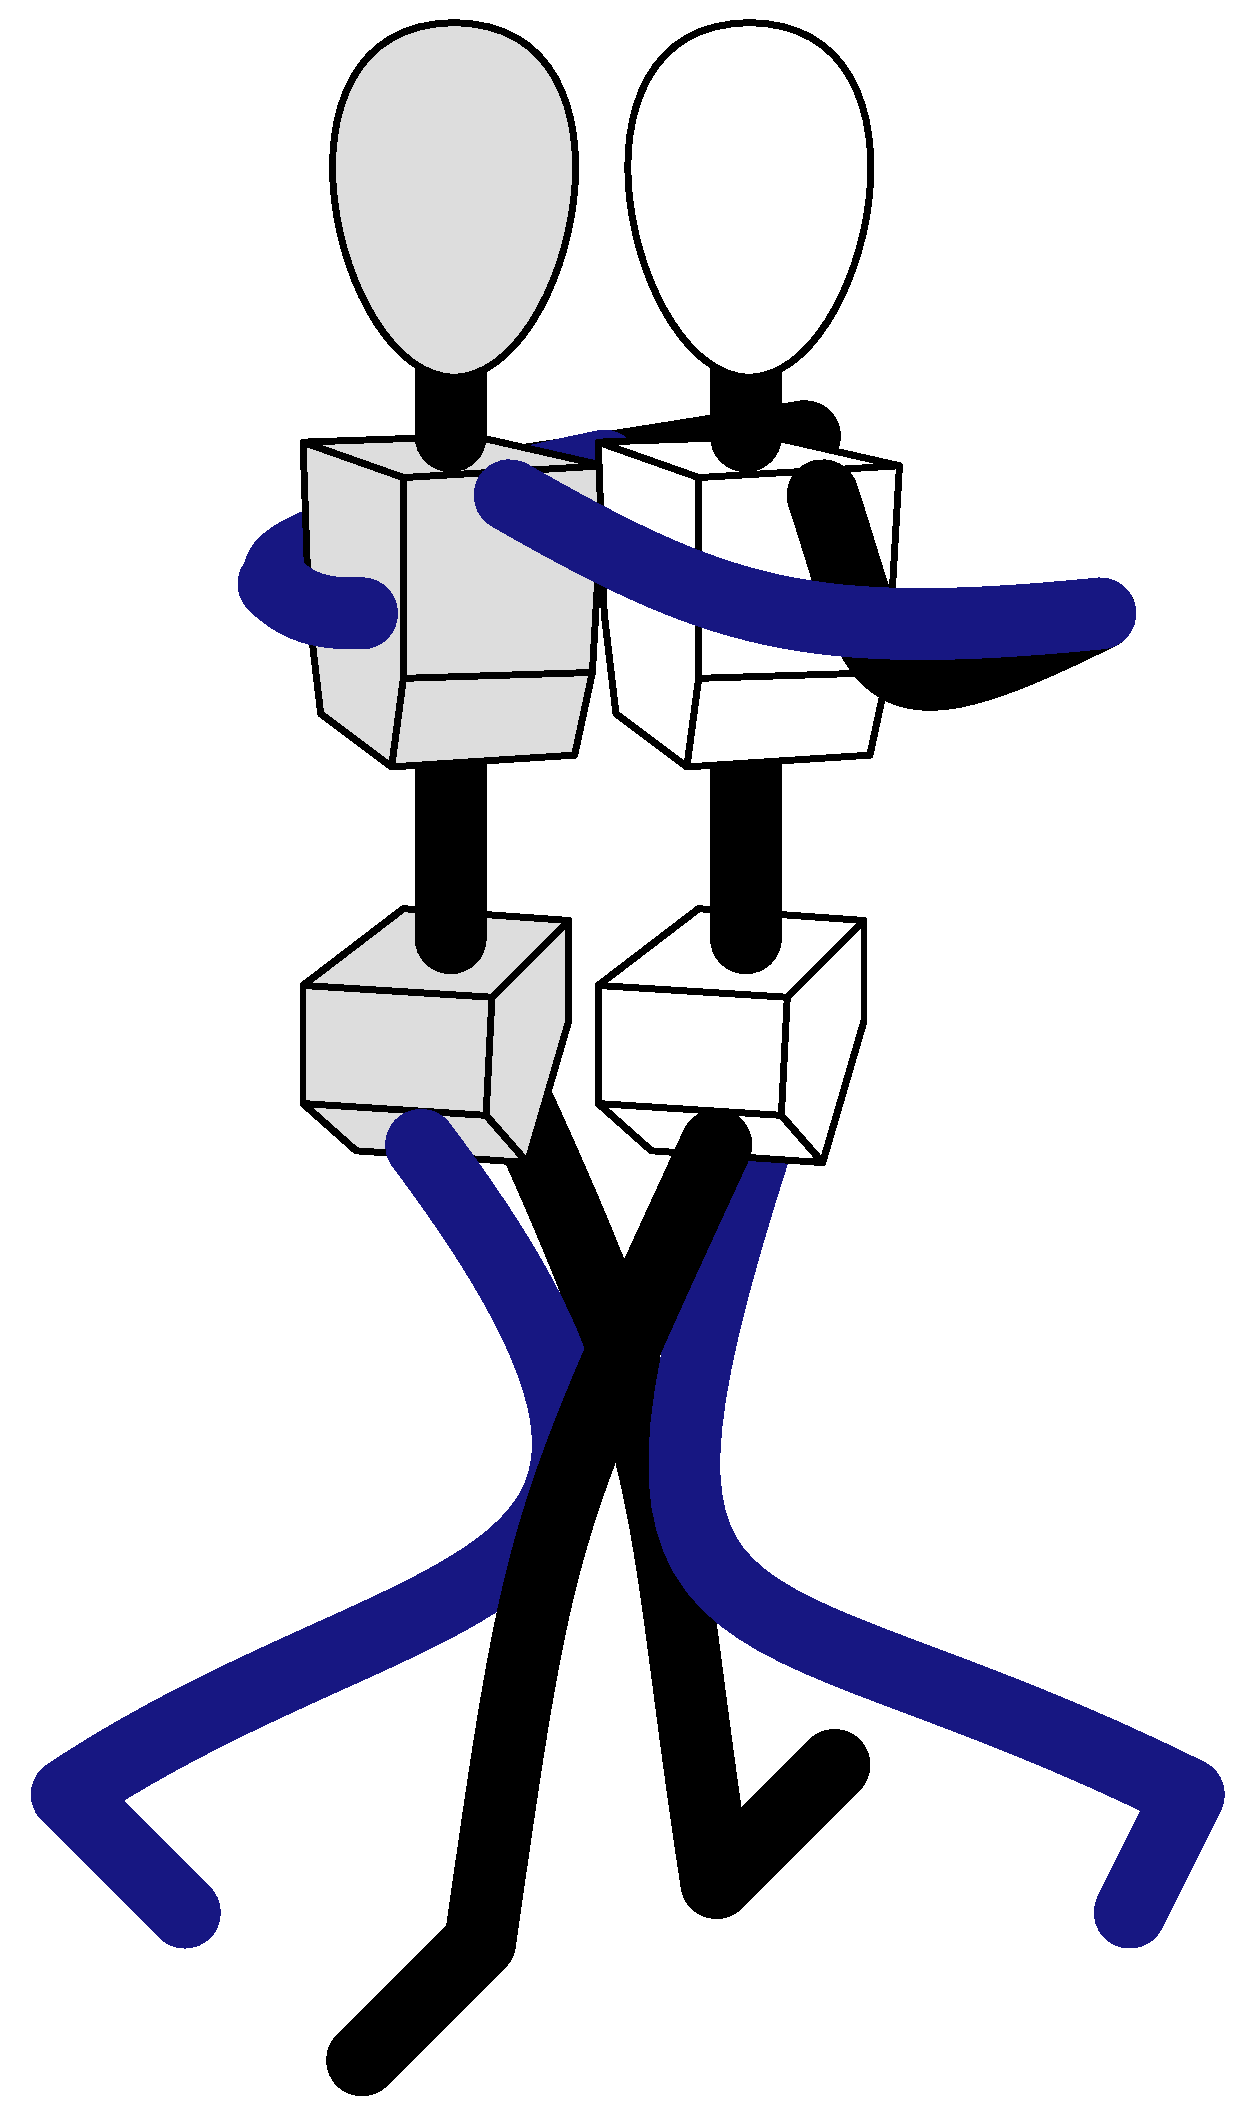
\includegraphics[width=0.23\textwidth]{chapters/cap-historia-passos/facao.eps}
  \caption{Pose final do facão.}
  \label{fig:facaostickman}
  \vspace{-10pt}
\end{wrapfigure}
Voltando ao facão de \AnoLivro, pessoalmente entendo mais este como uma posição que 
como um movimento ou passo. 
Isto é porque existem varias formas pra chegar à \hyperref[def:facao-position]{\textbf{posição de facão}},
de modo que é difícil apontar uma delas para assumir o nome de facão sobre as outras.

A posição do facão, é uma onde o par de dança está num abraçado colado e frente a frente, 
de modo que ambos tem a perna direita um pouco atrás do \hyperref[def:PlanoFrontal]{\textbf{plano frontal}} da linha da cabeça,
e a perna esquerda um pouco adiante no mesmo plano; com esta descrição se deduz 
que ambos tem o peso do corpo dividido em ambos pés; pelo que esta postura,
deve entende-se como uma de descanso, momentâneo porem descanso;
é dizer, se nossa dança fosse um relato escrito, a posição do facão
representaria um ponto, ou em alguns casos um ponto e virgula.
Se o que pretendemos representar é um ponto e virgula, 
é interessante não dividir o peso do corpo 50\% e 50\% em ambos pés,
e sim carregar o peso do corpo um pouco mais em um 
para poder liberar facilmente u outro pé para poder sair elegantemente da posição de facão.  

Sobre as formas de chegar a posição de facão, a continuação será descrita a forma mais simples,
porem não a mais interessante. Iniciamos desde o passo, frente-trás também chamado básico, 
ou básico linear no samba de gafieira. Desde o ponto de vista do \hyperref[def:Condutor]{\textbf{condutor}}, 
com um \hyperref[def:abracodedanca]{\textbf{abraço de dança}} colado,
damos primeiro duas pisadas no lugar, iniciando com a perna esquerda no tempo 1, e logo a perna direita no tempo 1.5,
logo damos um passo atrás com a perna direita no tempo 2; 
finalmente no tempo 3 damos mais um passo atrás com a perna direita, 
e se temos mantido o abraço colado, 
o \hyperref[def:Seguidor]{\textbf{seguidor}} sentirá a necessidade de dar um passo a frente com a perna esquerda,
chegando ambos à posição de facão.  

Este movimento linear para atrás e pouco interessante para chegar ao facão, mas pode ser apimentado,
se usamos um movimento sinuoso para atrás (em vez de um linear), este movimento,
é promovido pelo condutor, e tem forma de ``S'' onde a ligeira curva para a esquerda é realizada no tempo 1 e 1.5,
no tempo  2 chegamos ao ponto neutro o meio, onde a curva esta sobre a linha reta, e para chegar a 3, 
que também está sobre a linha reta e ao final de ambas curvas,
o condutor promove a curva para a sua direita.

%%%%%%%%%%%%%%%%%%%%%%%%%%%%%%%%%%%%%%%%%%%%%%%%%%%%%%%%%%%%%%%%%%%%%%%%%%%%%%%
\subsection{Faquinha}
\index{Passo!Faquinha}
\index{Passo de deslocamento!Faquinha}
\index{Passo cíclico!Faquinha}
%%                CICLICO     |SIMETRICO   |CONTRATEMPO   |DESLOCAMENTOS |TIEMPOS
\caracterpasso{\CheckedItem}{\NoCheckedItem}{\NoCheckedItem}{\CheckedItem}{2}
Este passo foi  criado entre o final da década de 1980 e inícios de 1990  \cite[pp. 143]{perna2002samba}.
É uma variante do  \hyperref[subsec:desc:passo:facao]{\textbf{facão}} (passo), 
com a diferencia que o movimento tem uma posição final (facão) menos acentuada;
sendo mais parecido a um casal num \hyperref[def:abracodedanca]{\textbf{abraço de dança}} colado, 
na \hyperref[def:frente-frente-position]{\textbf{posição frente a frente}}  e com uma perna ligeiramente adiantada a outra;
com diferencia da \hyperref[def:facao-position]{\textbf{posição de facão}}, 
onde as pernas tem uma separação que claramente evidencia uma posição do descanso;
a faquinha, pelo contrario, termina numa posição final de transição, 
pois comumente são realizadas varias faquinhas de forma consecutiva antes de realizar um facão,
 para assim finalizar a sequencia de forma mais acentuada.

O passo faquinha dura dois tempos, e consta de dois movimentos, 
onde a posição final é igual à inicial de modo que o passo pode repetir-se ciclicamente indefinidamente.
O movimento inicia quando o par de dança está numa posição de facão pouco acentuada;
é dizer, quando cada um tem pouca separação entre os pés; 
e o peso do corpo está do lado da perna direita do \hyperref[def:Condutor]{\textbf{condutor}}.
Logo, no primeiro tempo, 
o condutor junta os pés trazendo sua pé esquerdo junto à direito e trocando o peso do corpo a esse pé,
mantendo o abraço para provocar um movimento simétrico no \hyperref[def:Seguidor]{\textbf{seguidor}};
porem a ação do movimento dos pés não é uma causa e sim um efeito,
pois é provocado por uma condução do tórax usando que é transmitida por médio do abraço colado;
para isto o condutor gira o tórax no sentido horário no \hyperref[def:PlanoAxial]{\textbf{plano axial}},
tentando suspender ligeiramente o corpo do seguidor e o seu próprio.
No segundo tempo, o condutor dá um passo atrás com sua perna direita,
 mantendo o abraço colado e provocando que o seguidor de um passo adiante com sua perna esquerda,
chegando novamente a posição inicial.



%%%%%%%%%%%%%%%%%%%%%%%%%%%%%%%%%%%%%%%%%%%%%%%%%%%%%%%%%%%%%%%%%%%%%%%%%%%%%%%
\subsection{\textcolor{blue}{Gancho}} 
\index{Passo!Gancho}
Este passo foi  criado entre o final da década de 1980 e inícios de 1990  \cite[pp. 143]{perna2002samba}.

%%%%%%%%%%%%%%%%%%%%%%%%%%%%%%%%%%%%%%%%%%%%%%%%%%%%%%%%%%%%%%%%%%%%%%%%%%%%%%%
\subsection{\textcolor{blue}{Gancho redondo}} 
\index{Passo!Gancho redondo}
Este passo foi  criado entre o final da década de 1980 e inícios de 1990  \cite[pp. 143]{perna2002samba}.

%%%%%%%%%%%%%%%%%%%%%%%%%%%%%%%%%%%%%%%%%%%%%%%%%%%%%%%%%%%%%%%%%%%%%%%%%%%%%%%
\subsection{\textcolor{blue}{Letra}}
\index{Passo!Letra}
Este passo foi  criado entre o final da década de 1980 e inícios de 1990  \cite[pp. 143]{perna2002samba}.

%%%%%%%%%%%%%%%%%%%%%%%%%%%%%%%%%%%%%%%%%%%%%%%%%%%%%%%%%%%%%%%%%%%%%%%%%%%%%%%
\subsection{\textcolor{blue}{Puladinho redondo}} 
\index{Passo!Puladinho redondo}
Este passo foi  criado entre o final da década de 1980 e inícios de 1990  \cite[pp. 143]{perna2002samba}.

%%%%%%%%%%%%%%%%%%%%%%%%%%%%%%%%%%%%%%%%%%%%%%%%%%%%%%%%%%%%%%%%%%%%%%%%%%%%%%%
\subsection{\textcolor{blue}{Trança}}
\index{Passo cíclico!Trança}
\index{Passo!Trança}
Este movimento é antigo, porem Jaime Arôxa trabalhou sobre ele entre os anos de 1987 a 1990,
pois não existia uma didática para o ensino do movimento, 
e era realizado apenas pelos homens; 
de modo que Jaime agregou a parte do seguidor no par de dança  \cite{EntrevistaJaimeAroxa1} \cite[pp. 143]{perna2002samba}.
%%%%%%%%%%%%%%%%%%%%%%%%%%%%%%%%%%%%%%%%%%%%%%%%%%%%%%%%%%%%%%%%%%%%%%%%%%%%%%%
\subsection{\textcolor{blue}{Tesoura}}
\index{Passo!Tesoura}
Movimento criado por Jaime Arôxa, entre os anos de 1987 a 1990 \cite{EntrevistaJaimeAroxa1} \cite[pp. 143]{perna2002samba}.

%%%%%%%%%%%%%%%%%%%%%%%%%%%%%%%%%%%%%%%%%%%%%%%%%%%%%%%%%%%%%%%%%%%%%%%%%%%%%%%
%%%%%%%%%%%%%%%%%%%%%%%%%%%%%%%%%%%%%%%%%%%%%%%%%%%%%%%%%%%%%%%%%%%%%%%%%%%%%%%
\PRLsep{Passos de samba de gafieira da décadas de 1990}

%%%%%%%%%%%%%%%%%%%%%%%%%%%%%%%%%%%%%%%%%%%%%%%%%%%%%%%%%%%%%%%%%%%%%%%%%%%%%%%
\subsection{\textcolor{blue}{Assalto}} 
\index{Passo!Assalto}
\index{Passo cíclico!Assalto}
Este passo foi criado por Jimmy de Oliveira apos o ano 1990 \cite{sambafunkeadoJimmyDeOliveiraPart1}.

%%%%%%%%%%%%%%%%%%%%%%%%%%%%%%%%%%%%%%%%%%%%%%%%%%%%%%%%%%%%%%%%%%%%%%%%%%%%%%%
\subsection{\textcolor{blue}{Boneca}} 
\index{Passo!Boneca}
Este passo foi criado por Jimmy de Oliveira apos o ano 1990 \cite{sambafunkeadoJimmyDeOliveiraPart1}.

%%%%%%%%%%%%%%%%%%%%%%%%%%%%%%%%%%%%%%%%%%%%%%%%%%%%%%%%%%%%%%%%%%%%%%%%%%%%%%%
\subsection{\textcolor{blue}{Elástico}} 
\index{Passo!Elastico}
Este passo foi criado por Jimmy de Oliveira apos o ano 1990 \cite{sambafunkeadoJimmyDeOliveiraPart1}.

%%%%%%%%%%%%%%%%%%%%%%%%%%%%%%%%%%%%%%%%%%%%%%%%%%%%%%%%%%%%%%%%%%%%%%%%%%%%%%%
\subsection{\textcolor{blue}{Escovinha}}
\index{Passo cíclico!Escovinha}
\index{Passo!Escovinha}
Este passo foi criado por Jimmy de Oliveira apos o ano 1990 \cite{sambafunkeadoJimmyDeOliveiraPart1}.

%%%%%%%%%%%%%%%%%%%%%%%%%%%%%%%%%%%%%%%%%%%%%%%%%%%%%%%%%%%%%%%%%%%%%%%%%%%%%%%
\begin{comment}
\subsection{Homem na lua}
Este passo foi criado por Jimmy de Oliveira apos o ano 1990 \cite{sambafunkeadoJimmyDeOliveiraPart1}.
\end{comment}

%%%%%%%%%%%%%%%%%%%%%%%%%%%%%%%%%%%%%%%%%%%%%%%%%%%%%%%%%%%%%%%%%%%%%%%%%%%%%%%
\subsection{\textcolor{blue}{Pescaria}} 
\index{Passo!Pescaria}
Este passo foi criado por Jimmy de Oliveira apos o ano 1990 \cite{sambafunkeadoJimmyDeOliveiraPart1}.

%%%%%%%%%%%%%%%%%%%%%%%%%%%%%%%%%%%%%%%%%%%%%%%%%%%%%%%%%%%%%%%%%%%%%%%%%%%%%%%
\subsection{\textcolor{blue}{Romário}}
\label{subsec:passo:romario}
\index{Passo cíclico!Romário} 
\index{Passo!Romário}
Este passo foi criado por Jimmy de Oliveira apos o ano 1990 \cite{sambafunkeadoJimmyDeOliveiraPart1}.


%%%%%%%%%%%%%%%%%%%%%%%%%%%%%%%%%%%%%%%%%%%%%%%%%%%%%%%%%%%%%%%%%%%%%%%%%%%%%%%
%%%%%%%%%%%%%%%%%%%%%%%%%%%%%%%%%%%%%%%%%%%%%%%%%%%%%%%%%%%%%%%%%%%%%%%%%%%%%%%
\PRLsep{Passos de samba de gafieira sem data conhecida}



%%%%%%%%%%%%%%%%%%%%%%%%%%%%%%%%%%%%%%%%%%%%%%%%%%%%%%%%%%%%%%%%%%%%%%%%%%%%%%%
\subsection{\textcolor{blue}{Balanço}}
\index{Passo!Balanço}
\index{Passo cíclico!Balanço}
Movimento sem data de criação conhecida, 
seguindo Jaime Arôxa o balanço sempre existiu desde do início do século, 
no maxixe \cite{EntrevistaJaimeAroxa1},
sendo este um movimento considerado de nível básico \cite[pp. 144]{perna2002samba}.


%%%%%%%%%%%%%%%%%%%%%%%%%%%%%%%%%%%%%%%%%%%%%%%%%%%%%%%%%%%%%%%%%%%%%%%%%%%%%%%
\subsection{\textcolor{blue}{Saída lateral}}
\index{Passo!Saída lateral}
Movimento sem data de criação conhecida,
sendo este um movimento considerado de nível básico \cite[pp. 144]{perna2002samba}.

%%%%%%%%%%%%%%%%%%%%%%%%%%%%%%%%%%%%%%%%%%%%%%%%%%%%%%%%%%%%%%%%%%%%%%%%%%%%%%%
\subsection{\textcolor{blue}{Tirada ao lado}}
\index{Passo!Tirada ao lado}
Movimento sem data de criação conhecida,
sendo este um movimento considerado de nível básico \cite[pp. 144]{perna2002samba}.

%%%%%%%%%%%%%%%%%%%%%%%%%%%%%%%%%%%%%%%%%%%%%%%%%%%%%%%%%%%%%%%%%%%%%%%%%%%%%%%
\begin{comment}
\subsection{\textcolor{blue}{Mestre sala}}
\index{Passo!Mestre sala}
Movimento sem data de criação conhecida \cite[pp. 144]{perna2002samba}.
\end{comment}


%%%%%%%%%%%%%%%%%%%%%%%%%%%%%%%%%%%%%%%%%%%%%%%%%%%%%%%%%%%%%%%%%%%%%%%%%%%%%%%
\begin{comment}
\subsection{\textcolor{blue}{Enceradeira}}
\index{Passo!Enceradeira}
Movimento sem data de criação conhecida \cite[pp. 144]{perna2002samba}.
\end{comment}



%%%%%%%%%%%%%%%%%%%%%%%%%%%%%%%%%%%%%%%%%%%%%%%%%%%%%%%%%%%%%%%%%%%%%%%%%%%%%%%
%%%%%%%%%%%%%%%%%%%%%%%%%%%%%%%%%%%%%%%%%%%%%%%%%%%%%%%%%%%%%%%%%%%%%%%%%%%%%%%

\begin{comment}
Passos acrobáticos ou para apresentações \cite[pp. 142-143]{perna2002samba}:
\begin{tasks}
\task \textbf{Cabide}, \index{Passo!Cabide} oriundo do rock.
\task \textbf{Baratinha} \index{Passo!Baratinha}
\task \textbf{Enceradeira}, \index{Passo!Enceradeira} criado em algum momento no final da década de 1980 e inícios da década de 1990.
\end{tasks}
\end{comment}
